% !TEX root = ../main.tex
% 第二日第一讲：TQFT 续论、自守理论、Hecke 算子
\section{第二日第一讲}

\subsection{TQFT 续论}
上一次（第一日第一讲）我们讲了 TQFT 的概念，把它当作把到 $BG=\bullet/G$ 的映射线性化的手段。
在第一日第三讲里我们考虑过 $|G|<\infty$ 的例子：一个 TQFT $A_G$ 连同场的数据 $\mathcal F_G$，使得
\[
  \mathcal F_G(C)=\Bun_G(C)=\Maps(C,\bullet/G)=\Hom(\pi_1(C),G)/G.
\]
注意在 $G$ 有限的前提下，$\Loc_G(\Sigma)=\Bun_G(\Sigma)=\Maps(\Sigma,\bullet/G)$，本节里我们随意地这样假定。
例如
\[
  \mathcal F_G(S^1)=\Maps(S^1,\bullet/G)=\Hom(\mathbb Z,G)/G=G/G,
\]
其中商是对共轭作用取的。

我们也可以把 $\bullet/G$ 换成一个有限群胚（栈）$X=X/G$，其中 $X$ 是 $G$-空间，并取 $\mathcal F_G$ 为
\[
  \mathcal F_G(S^1)=\Loc^X_G(S^1)=\Bun^X_G(S^1)=\Maps(S^1,X/G)
  =\{x\in X,\ g\in G,\ g\cdot x=x\}/G
\]
（把 $S^1$ 换成一般的 $\Sigma$ 也类似）。

注意有一个由 $X/G\to\bullet/G$ 诱导的映射 $\Loc^X_G(\Sigma)\to\Loc_G(\Sigma)$，因为 $\Loc_G(\Sigma)=\Maps(\Sigma,\bullet/G)\,(=\Bun_G(\Sigma))$。
一旦固定了这样的 $G$-空间 $X$，我们就有一个杰出元
\[
  \Theta_{G,X}(\Sigma)\in Z^3_G(\Sigma)=\mathbb C[\Loc_G(\Sigma)],
\]
它定义一个边界理论 $\Theta_{G,X}$。

4 维（算术）TQFT $Z=A_G$ 可以通过先取场 $\mathcal F_G=\Bun_G(-)=\Maps(-,\bullet/G)$、再线性化（取空间上的函数/层）得到，其抽象说法如下图所示：
\[
\begin{array}{ccc}
\text{流形}/\!\!\text{ 配边} & \xrightarrow{\quad A_G\quad} & \text{线性范畴}/\!\!\text{ 态射}\\[2pt]
\searrow^{\ \mathcal F_G} & & \nearrow_{\ \text{取函数/层}}\\[2pt]
& \text{群胚（栈）}/\!\!\text{ 对应} &
\end{array}
\]

我们来讨论 $A_G$ 的函子性。
我们知道 $A_G$ 经 $\mathcal F_G$ 因子化，所以先描述 $\mathcal F_G$ 的函子性。
给定配边
\[
  M:\partial_{\mathrm{in}}\to\partial_{\mathrm{out}},
\]
由下面的图得到一种对应
\[
\begin{array}{ccc}
& \mathcal F_G(M)=\Bun_G(M) &\\[2pt]
\swarrow_{\ f} & & \searrow^{\ g}\\[2pt]
\mathcal F_G(\partial_{\mathrm{in}})=\Bun_G(\partial_{\mathrm{in}}) & &
\mathcal F_G(\partial_{\mathrm{out}})=\Bun_G(\partial_{\mathrm{out}}).
\end{array}
\]
然后，沿第一个映射 $f$ 拉回、沿第二个映射 $g$ 前推，就得到态射 $A_G(M):A_G(\partial_{\mathrm{in}})\to A_G(\partial_{\mathrm{out}})$。

此外，给定 $G$-空间 $X$ 时，我们可以定义杰出对象 $\Theta_{G,X}(\Sigma)\in A_G(\Sigma)$。
取一个扩张配边 $M:\emptyset\to\Sigma$（图 4.1）即可得。

\insfig[0.30\textwidth]{f41-empty}{$M:\emptyset\to\Sigma$}

它给出对应
\[
\begin{array}{ccc}
& \Bun^X_G(\Sigma)=\Maps(\Sigma,X/G) &\\[2pt]
\swarrow & & \searrow\\[2pt]
\mathcal F_G(\emptyset)=\bullet & & \mathcal F_G(\Sigma)=\Maps(\Sigma,\bullet/G),
\end{array}
\]
进而给出一个态射 $1\to A_G(\Sigma)$，等价地说，给出 $A_G(\Sigma)$ 中的一个对象 $\Theta_{G,X}(\Sigma)$。
我们就是这样得到周期函数/周期层的（在 B 侧（谱侧）类似地得到 L-函数/L-层）。

\subsection{自守理论}
现在考虑 $G$ 是域 $k$ 上的约化群的情形，得到推广到算术流形的 4 维 TQFT $A_G$。
$A_G$ 由代数 $G$-丛的模空间的拓扑构成。

在整体几何设定中：$\Sigma$ 是 $F=\overline F$（例如 $\mathbb C$、$\overline{\mathbb F}_q$）上的代数曲线（2 维），于是得到 $\mathcal F_{A_G}(\Sigma)=\Bun_G(\Sigma)$。

\begin{exmp}
$\mathcal F_{\mathbb G_m}(\Sigma)=\Pic(\Sigma)$。
\end{exmp}

\begin{exmp}
若 $\Sigma=D^\times_F=\Spec(F((t)))$，则
\[
  \mathcal F_G(D^\times_F)=\Bun_G(D^\times_F)=\bullet/G(F((t))).
\]
\end{exmp}

\begin{exmp}
若 $\Xi$ 是 $\mathbb F_q$ 上的曲线，则
\[
  \mathcal F_G(\Xi)=\Bun_G(\Sigma)^{\Frob}=\Bun_G(\Sigma)(\mathbb F_q).
\]
（这里 $\Sigma$ 是 $\Xi$ 基变换到 $\overline{\mathbb F}_q$ 所得，$\Bun_G(\Sigma)^{\Frob}$ 是关于 Frobenius 的不动点空间。）
\end{exmp}

\begin{exmp}
特别地，若 $\Sigma=D^\times_{\mathbb F_q}=\Spec(\mathbb F_q((t)))$，则
\[
  \mathcal F_G(D^\times_{\mathbb F_q})=\Bun_G\bigl(D^\times_{\mathbb F_q}\bigr)^{\Frob}
  =G(\mathbb F_q((t)))/^{\Frob}G(\mathbb F_q((t)))\supset\bullet/G(\mathbb F_q((t))).
\]
\end{exmp}

现在我们要把上述空间线性化。
注意 $A_G$ 把 3 维流形送到向量空间，把 2 维流形送到线性范畴。

\begin{exmp}
对例 4.3 中的 3 维流形 $\Xi$，有
\[
  A_G(\Xi)=\Fun(\Bun_G(\Sigma)(\mathbb F_q)),
\]
即无分歧自守形式的向量空间。
\end{exmp}

\begin{exmp}
对例 4.4 中的 2 维流形 $D^\times_{\mathbb F_q}$，有
\[
  A_G(D^\times_{\mathbb F_q})=\Shv(\Bun_G(D^\times_{\mathbb F_q}))
  =\Shv\bigl(G(\mathbb F_q((t)))/^{\Frob}G(\mathbb F_q((t)))\bigr),
\]
即与穿孔圆盘相伴的自守范畴；它包含 $\Shv(\bullet/G(\mathbb F_q((t))))=\Rep^{\mathrm{smooth}}(G(\mathbb F_q((t))))$，即该局部域 $\mathbb F_q((t))$ 上的群的平滑表示范畴，也就是经典局部 Langlands 所研究的对象。
\end{exmp}

\begin{exmp}
人们可能以为 TQFT 只编码无分歧部分的信息，但其实它也能看见分歧部分：

\inlfig[0.86\textwidth]{f44-ramified}

我们有 $\Spec(\mathbb Z[1/2])$，把它看作以 $\Spec(\mathbb Q_2)$ 与 $\Spec(\mathbb R)$ 为两个边界分支的 3 维流形。
类似地，可以取有限域 $\mathbb F_q$ 上的曲线 $\Sigma$，挖掉几个点 $x_1,x_2$，然后看 $\Fun(\Bun_G(\Xi|x_1,x_2))$（$\Bun_G$ 上带两个点处某些额外数据的函数）。
这给出 $\Rep G(\mathbb F_q((t)))^2$ 中的一个对象。
细节从略，要点是：TQFT 当然知道如何处理分歧——我们只需挖掉一些东西，于是与闭 3 维流形得到向量空间不同，我们得到与边界相伴的范畴中的一个对象，此地即 $\Rep G(\mathbb F_q((t)))^2$。
\end{exmp}

下图这个菱形给出各种整体/局部、算术/几何设定的大图景：
\begin{center}
\begin{tikzpicture}[scale=0.78, every node/.style={font=\footnotesize}]
  \coordinate (T) at (0,2);
  \coordinate (L) at (-2.9,0);
  \coordinate (R) at (2.9,0);
  \coordinate (B) at (0,-2);
  \draw (T)--(L)--(B)--(R)--(T);
  \node[above] at (T) {$\mathbb Q,\ \Xi=\Sigma$（$\mathbb F_q$ 上）};
  \node[left]  at (L) {$\mathbb Q_p,\ \mathbb F_q((t))$};
  \node[right] at (R) {$\Sigma$（$\mathbb C$、$\overline{\mathbb F}_q$ 上）};
  \node[below] at (B) {$\overline{\mathbb F}_q((t)),\ \mathbb C((t))$};
  \node at (-1.75,1.5) {算术};
  \node at (1.75,1.5)  {整体};
  \node at (-1.75,-1.5) {局部};
  \node at (1.75,-1.5)  {几何};
  \node[right] at (7.0,2)  {3-流形};
  \node[right] at (7.0,0)  {2-流形};
  \node[right] at (7.0,-2) {1-流形};
\end{tikzpicture}
\end{center}

\begin{figure}[htbp]
\centering
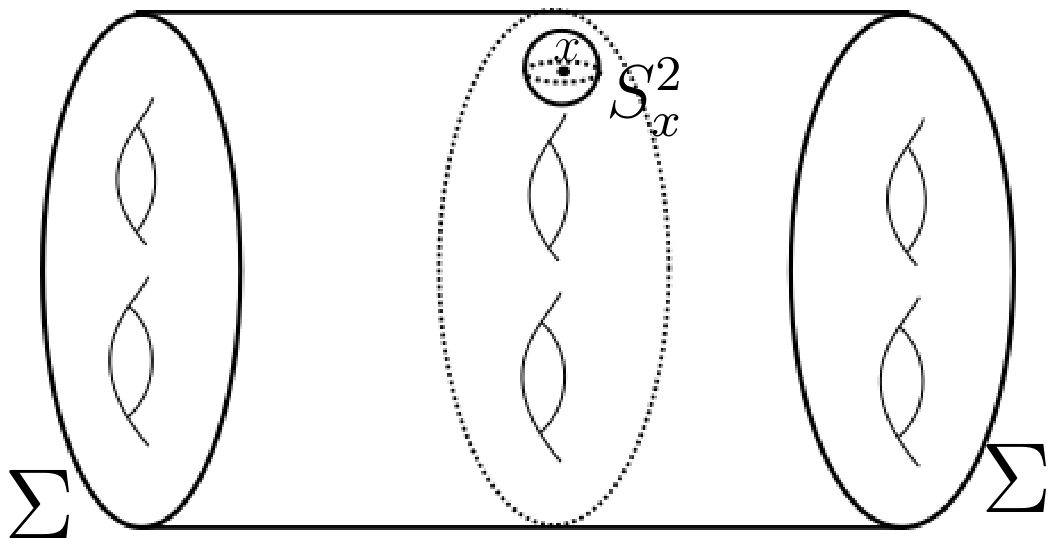
\includegraphics[width=0.72\textwidth]{f42-bordism}
\caption{配边 $(\Sigma\times I)\setminus D^3_x:S^2_x\sqcup\Sigma\to\Sigma$}
\label{fig:f42}
\end{figure}

我们还没有明确所用的层论是什么。
例如，对整体几何 Langlands，有
\[
  A_G(\Sigma)=\Shv^?_N(\Bun_G(\Sigma)),\qquad
  ?=\begin{cases}
    \mathrm{dR}\ (\text{de Rham}), & \text{D-模},\\
    \mathrm{B}\ (\text{Betti}), & \text{向量空间层},\\
    \text{ét}\ (\text{étale}), & \text{平展可构造层}.
  \end{cases}
\]
（确切地说，还需要一处技术性修正才能让一切成立：我们需要取具有幂零支撑的层。
例如当 $G=\mathbb G_m$ 时 $\Bun_G(-)=\Pic(-)$，「幂零支撑」这个形容词让我们只需处理 $\Pic$ 上的局部常值层，而不是所有层。）

\subsection{可观测量的对称性、Hecke 算子}
让我们回到有限群的设定。
设 $H$ 是有限群，于是 $\Bun_H(-)=\Loc_H(-)$。
考虑昨天讲过的与有限群 $H$ 相伴的 4 维 TQFT $Z^4_H$，使得 $Z^4_H(\Sigma)=\Vect(\Bun_H(\Sigma))$。
这个范畴有很好的对称性，并且被可观测量作用，即被 $Z^4_H(S^2)$（又称 Hecke 范畴/线算子范畴）作用，如昨天第一讲所解释。
这个作用可以通过把 $Z^4_H$ 作用于图 4.2 中的配边（选好 $x\in\Sigma$）得到：

具体地，
\[
  Z^4_H(S^2_x)=\Vect(\bullet/H)=(\Rep(H),\otimes)
\]
（因为 $\Bun_H(S^2)=\Loc_H(S^2)=\bullet/H$），它如下作用于 $Z^4_H(\Sigma)$：
\begin{itemize}[leftmargin=2.0em,itemsep=0.3em]
\item 对每个 $x\in\Sigma$，有映射
\[
  \Bun_H(\Sigma)\xrightarrow{\ (-)|_x\ }\Bun_H(x)=\bullet/H;
\]
\item 给定 $V\in Z^4_H(S^2)=\Rep(H)$，沿上述映射把它拉回，得到 $\Bun_H(\Sigma)$ 上的向量丛 $V_x$。
\end{itemize}

\begin{figure}[htbp]
\centering
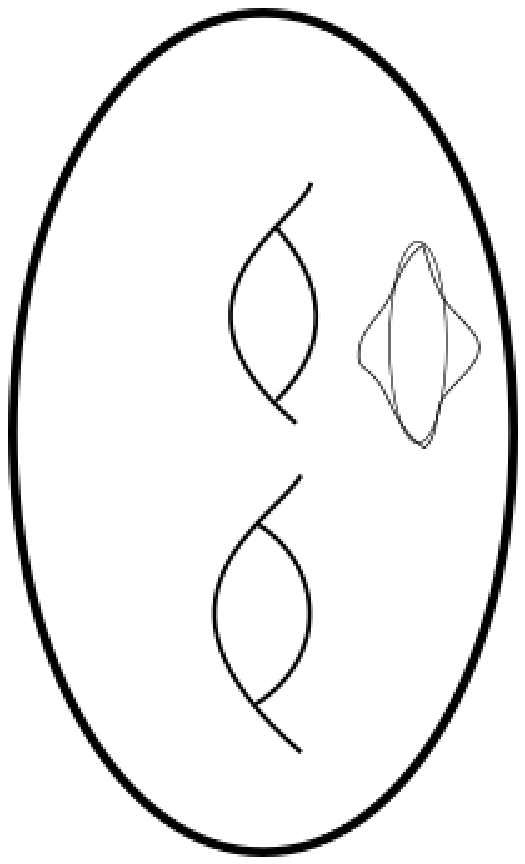
\includegraphics[width=0.24\textwidth]{f43-raviolo}
\caption{$\Sigma\sqcup_{\Sigma\setminus\{x\}}\Sigma
=\Sigma\sqcup_{D_x}\bigl(\text{raviolo}\bigr)
=\Sigma\sqcup_{D_x}\bigl(D_x\sqcup_{D^\times_x}D_x\bigr):\Sigma\to\Sigma$}
\label{fig:f43}
\end{figure}

\begin{itemize}[leftmargin=2.0em,itemsep=0.3em]
\item 于是 $V$ 通过下式作用于 $E\in Z^4_H(\Sigma)$：
\[
  V\cdot E:=V_x\otimes E.
\]
\end{itemize}

我们在 Langlands 对应的 B 侧（谱侧）将要看到的算子，正是这个样子的。

现在回到 $G$ 是约化群的情形。
取
\[
  Z(-)=A_G(-)=\Shv^?_N(\Bun_G(-))
\]
（或者可以取与圆的乘积再取 Frobenius 的迹；对有限域上的曲线，我们把层换成自守函数）。

要得到 Hecke 算子，我们再次取 $x\in\Sigma$，并看配边（图 4.2）。
取场空间之后，这本应给出一个对应，再线性化就得到 Hecke 作用。
但当然，由于技术上的困难我们不能直接这样做：$I=[0,1]$ 不是代数曲线，所以必须弄清如何在代数几何中解读这一点。
既然一切都应当是局部常值的，可以想象把这张图收缩，得到某个像「$\Sigma$ 沿 $x$ 处的圆盘与一个 raviolo 粘起来」的东西（见下图 4.3）。
raviolo 应看作 $D\sqcup_{D^\times}D$，是扮演 2-球面角色的代数几何对象。

取场空间之后就得到对应，即 Hecke 对应：
\[
\begin{array}{ccc}
& \Bun_G(\Sigma\sqcup_{\Sigma\setminus\{x\}}\Sigma)=\mathrm{Hecke}_x &\\[2pt]
\swarrow & & \searrow\\[2pt]
\Bun_G(\Sigma) & & \Bun_G(\Sigma).
\end{array}
\]
这里 $\Bun_G(\Sigma\sqcup_{\Sigma\setminus\{x\}}\Sigma)$ 的元素，无非是在 $x$ 之外等同起来的一对 $G$-丛，但也可以看作 $\Sigma$ 上的单个 $G$-丛连同 $x$ 处局部修改的某些局部数据。
现在取自守函数/层，沿第一个映射拉回、乘/张量上 $A_G(\text{raviolo})$ 中的某个东西、再沿第二个映射前推，就得到算子/函子。
这就给出 $A_G(\text{raviolo})$ 在 $A_G(\Sigma)$ 上的 Hecke 作用。

\begin{exmp}
\leavevmode\par
\begin{itemize}[leftmargin=2.0em,itemsep=0.3em]
\item （算术设定，来自第一日第二讲）回忆在算术语境中，Hecke 算子的作用是这样得到的：取与数域相伴的对象，挖掉一个素点（即把该素点反转），再把它粘回去，于是得到粘回去的那个东西的自同态。
该设定中的 Hecke 作用可以看作恰好来自上面的配边。
\item 若 $G=\mathbb G_m$，则 $\Bun_G(D_x\sqcup_{D^\times_x}D_x=:\text{raviolo})=\mathbb C((t))^\times/\mathbb C[[t]]^\times\cong\mathbb Z$，而 $A_G(\text{raviolo})=\Shv(\mathbb Z)$ 在 $A_G(\Sigma)=\Shv(\Pic(\Sigma))$ 上的 Hecke 作用，本质上由 $\mathbb Z$ 在 $\Pic(\Sigma)$ 上的作用 $n:L\mapsto L(nx)$ 诱导。
\end{itemize}
\end{exmp}
